\section{Qt}

\begin{figure}[H]
	\centering 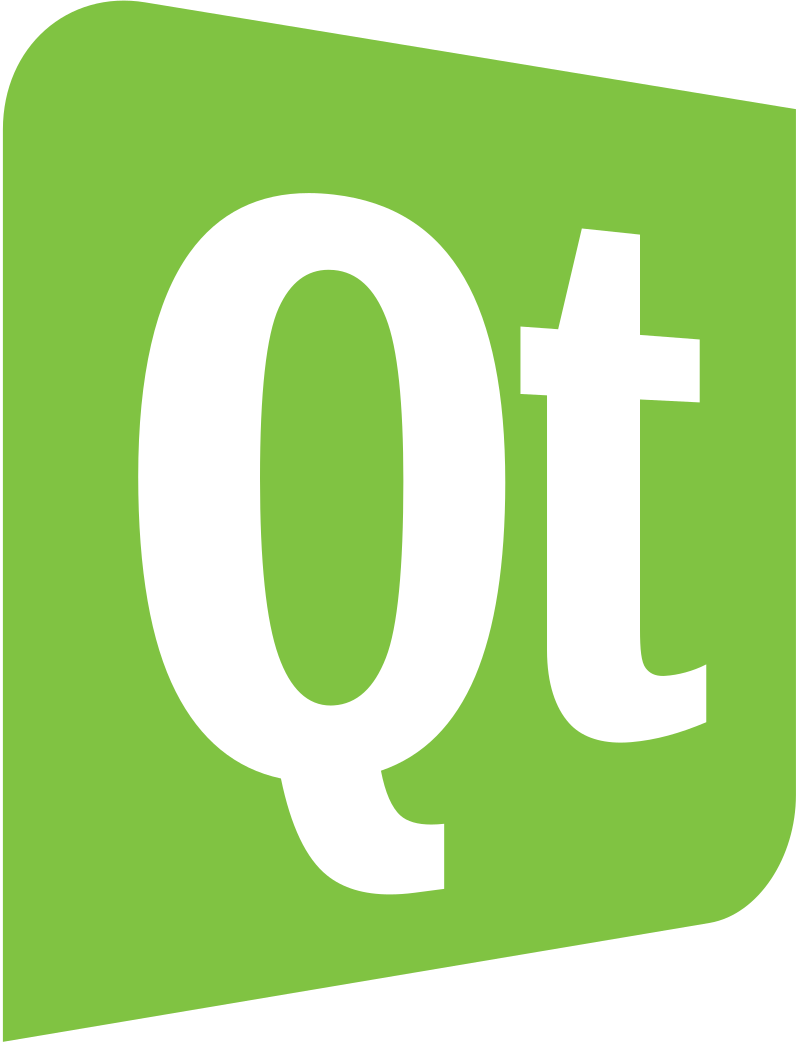
\includegraphics[scale=0.1]{images/qt.png}
	\caption{Qt Logo}
\end{figure}

Qt is a cross-platform application framework that is widely used for developing application software that can be run on various software and hardware platforms with little or no change in the underlying codebase, while still being a native application with native capabilities and speed. Qt is currently being developed both by The Qt Company, a company listed on the Nasdaq Helsinki Stock Exchange and the Qt Project under open-source governance, involving individual developers and firms working to advance Qt. Qt is available with both commercial and open source GPL 2.0, GPL 3.0, and LGPL 3.0 licenses.

Qt is used mainly for developing application software with graphical user interfaces (GUIs); however, programs without a GUI can be developed, such as command-line tools and consoles for servers. An example of a non-GUI program using Qt is the Cutelyst web framework. GUI programs created with Qt can have a native-looking interface, in which case Qt is classified as a widget toolkit.

Qt uses standard C++ with extensions including signals and slots that simplify handling of events, and this helps in development of both GUI and server applications which receive their own set of event information and should process them accordingly. Qt supports many compilers, including the GCC C++ compiler and the Visual Studio suite. Qt also provides Qt Quick, that includes a declarative scripting language called QML that allows using JavaScript to provide the logic. With Qt Quick, rapid application development for mobile devices became possible, although logic can be written with native code as well to achieve the best possible performance. Qt can be used in several other programming languages via language bindings. It runs on the major desktop platforms and some of the mobile platforms. It has extensive internationalization support. Non-GUI features include SQL database access, XML parsing, JSON parsing, thread management and network support.
\subsection{Software Architecture}
Qt, when it was first released, relied on a few key concepts:\\
\begin{itemize}
	\item \textbf{Complete abstraction of the GUI}: When first released, Qt used its own paint engine and controls, emulating the look of the different platforms it runs on when it drew its widgets. This made the porting work easier because very few classes in Qt depended really on the target platform; however, this occasionally led to slight discrepancies where that emulation was imperfect. Recent versions of Qt use the native style APIs of the different platforms, on platforms that have a native widget set, to query metrics and draw most controls, and do not suffer from such issues as much.[56] On some platforms (such as MeeGo and KDE) Qt is the native API. Some other portable graphical toolkits have made different design decisions; for example, wxWidgets uses the toolkits of the target platform for its implementations.
	\item \textbf{Signals and slots}: A language construct introduced in Qt for communication between objects which makes it easy to implement the observer pattern while avoiding boilerplate code. The concept is that GUI widgets can send signals containing event information which can be received by other controls using special functions known as slots.
	\item \textbf{Metaobject compiler}: The metaobject compiler, termed moc, is a tool that is run on the sources of a Qt program. It interprets certain macros from the C++ code as annotations, and uses them to generate added C++ code with meta information about the classes used in the program. This meta information is used by Qt to provide programming features not available natively in C++: signals and slots, introspection and asynchronous function calls.
\end{itemize}
\subsection{Qt Tools}
Qt comes with its own set of tools to ease cross-platform development, which can otherwise be cumbersome due to different set of development tools. Qt Creator is a cross-platform IDE for C++ and QML. Qt Designer's GUI layout/design functionality is integrated into the IDE, although Qt Designer can still be started as a standalone tool.\\
In addition to Qt Creator, Qt provides qmake, a cross-platform build script generation tool that automates the generation of Makefiles for development projects across different platforms. Without such a tool, one would have to write different Makefiles for each platform, so it is useful for abstracting away the differences of various platforms.\\
There are other tools available in Qt, including the Qt Designer interface builder and the Qt Assistant help browser (which are both embedded in Qt Creator), the Qt Linguist translation tool, uic (user interface compiler), and moc (Meta-Object Compiler).
